\documentclass[12pt,a4paper]{article}  % Déclare la classe du document.

\newcommand{\chaptermark}[2]{\og #2 \fg{} (#1)} % ligne uniquement pour éviter une erreur en cas d'article
\include{../1ere-preambule}
\usepackage{mathrsfs}

\usepackage{epic}   % extension et simplification de  l'environnement picture
\usepackage{graphicx}    % permet d'inclure des graphique externe dans un document
\usepackage{arydshln}   %permet d'avoir des lignes en pointillés

\newcommand{\lignes}[1]{
\setlength{\unitlength}{1mm}
\vskip 0,4cm\noindent
\multido{\i=0+1}{#1}{%
     \noindent
     \begin{picture}(150,5)
     \linethickness{0,005mm}
     \put(-5,0){\dashline{1}(175,5)(5,5)}
     \end{picture}\vskip 0,001cm
     }
\vskip 0cm
}

\rhead{DS n$^{\circ}$03 - 18/01/2023}

\begin{document}

\begin{center}
\fbox{
\begin{minipage}[]{15cm}
\begin{center}
\LARGE{\rule{0.5cm}{0pt}\rule[-0.25cm]{0pt}{0.9cm}
DS n$^{\circ}$3\\
Équations du second degré\\
}
\end{center}
\end{minipage}
}

\end{center}


\begin{center}\textbf{2 heures - Calculatrice autorisée - Barème indicatif}\end{center}

%\begin{center}\textbf{Les élèves avec un tier-temps ne traitent pas les questions avec  le symbole \ding{46}}\end{center}

\begin{center}
%On veillera à ENCADRER ses résultats et soigner sa copie.\\
Les résultats doivent être justifiés par des calculs (au moins 1 étape intermédiaire).
\end{center}
\vspace{.05cm} 

\vspace*{-0.5cm}
\exerciceDS{ - Equations - ( 3 points )}

Déterminer les racines des fonctions polynômes du second degré.
\begin{multicols}{2}
\begin{enumMet}
    \item $f(x)=3(x+7)(-x+11)$ \bareme{1}
    \item $g(x)=x(x-45)$ \bareme{1}
    \item $h(x)=-4(x+6)(x-501)$ \bareme{1}
\end{enumMet}
\end{multicols}

\vspace{-0.3cm}
\exerciceDS{ - Factorisation - ( 6 points )}

Donner les racines du polynôme du second degré donné, puis le factoriser
\begin{multicols}{2}
\begin{enumMet}
    \item $A(x)=x^{2}+6 x+9$ \bareme{1,5}
    \item $B(x)=\dfrac{2}{3}x^{2}-\dfrac{5}{7} x-\dfrac{3}{7}$ \bareme{1,5}
    \item $C(x)=x^{2}+18 x+77$ \bareme{1,5}
    \item $D(x)=2 x^{2}-7 x+8$ \bareme{1,5}
\end{enumMet}
\end{multicols}

\vspace{-0.3cm}
\exerciceDS{ - Inéquations - ( 8 points )}

Résoudre les inéquations données.
\begin{multicols}{2}
\begin{enumMet}
    \item $4 x^{2}-2 x+\dfrac{1}{4}>0$ \bareme{2}
    \item $x^{2}-3 x+5 \leqslant 0$ \bareme{2}
    \item $6 x^{2}+7 x-3 \geqslant 0$ \bareme{2}
    \item $49 x^{2}-4 \geqslant 0$ \bareme{2}
\end{enumMet}
\end{multicols}

\vspace{-0.3cm}
\exerciceDS{ - Tableau de variations - ( 2 points )}
Pour la fonction polynôme du second degré ci-dessous, dresser son tableau de variations (les valeurs du tableau de variations doivent être justifiées).
$$f(x)=-4x^2+22x+12$$

\vspace{-0.3cm}
\exerciceDS{ - Somme et Produit de racines - ( 3 points )}

Pour chaque équation, déterminer une solution évidente et en déduire l'autre sans calculer le discriminant.
\begin{multicols}{2}
\begin{enumMet}
    \item $3x^2-4x-7=0$ \bareme{1,5}
    \item $-2x^2+14x-20=0$ \bareme{1,5}
\end{enumMet}
\end{multicols}

\newpage

%\exerciceDS{ - Problème - ( 3 points )}
%
%Le sponsor d'une célèbre équipe de football vend des maillots aux couleurs de l'équipe.\\
%
%Il achète ces maillots à son fournisseur au prix de $10$ \EUR{} l'unité. Il en vend 200 unités par jour à $50$ \EUR{} chacune. Au vu des bons résultats de l'équipe au cours de la saison, il souhaite augmenter le prix de ces maillots.\\
%
%Il réalise une étude de marché qui montre que toute augmentation de $1$ \EUR{} fera baisser la vente de deux maillots par jour. On admet que le nombre de maillots achetés au fournisseur est le même que le nombre de maillots vendus, quel que soit le prix.\\
%
%\textbf{Déterminer le nouveau prix que devra fixer le sponsor pour réaliser un bénéfice maximum.}

\exerciceDS{ - Problème - ( 6 points )}
Une entreprise fabrique et vend des composants électroniques. Chaque composant est vendu 30 euros et l'entreprise en vend 1000 par semaine.\\
Une étude de marché a montré que pour chaque baisse de un euro du prix de vente unitaire, l'entreprise vendra 100 composants de plus par semaine.\\
Pour $x \in[0 ; 30]$, on note $R(x)$ le revenu réalisé par l'entreprise sur une semaine pour une baisse de $x$ euros du prix unitaire de vente.
\begin{enumMet}
	\item \begin{enumMet}
		\item Lorsque le prix de vente est de 30 \EUR{}, combien l'entreprise vent-elle de pièces et quel est la recette? \bareme{0,5}
		\item Lorsque le prix de vente est de 29 \EUR{}, combien l'entreprise vent-elle de pièces et quel est la recette? \bareme{0,5}
		\item Lorsque le prix de vente est de 28 \EUR{}, combien l'entreprise vent-elle de pièces et quel est la recette? \bareme{0,5}
	\end{enumMet}
	\item Montrer que $R(x)=100(10+x)(30-x)$. \bareme{1,5}
	\item Développer $R(x)$. \bareme{1}
	\item Écrire $R(x)$ sous forme canonique. \bareme{1}
	\item Déterminer le prix de vente unitaire que doit fixer l'entreprise pour que le revenu soit maximum. Quel est ce revenu maximum ? \bareme{1}
\end{enumMet}


\exerciceDS{ - Lien entre graphique et calcul - ( 3 points )}
On considère les fonctions $f$ et $g$, de courbes représentatives $\mathscr{C}_f$ et $\mathscr{C}_g$, définies sur $\mathbb{R}$ par:
$$
f(x)=2 x^2+2 x-3 \text { et } g(x)=-x^2-x+3
$$

\begin{enumMet}
	\item A l'aide de la calculatrice, tracer les courbes représentatives $\mathscr{C}_f$ et $\mathscr{C}_g$ des fonctions $f$ et $g$. En déduire la position relative des courbes. \bareme{1} %(Pour quels valeurs de $x$, $\mathscr{C}_f$ est au-dessus de $\mathscr{C}_g$).
%	\item On a tracé ci-dessous les courbes $\mathscr{C}_f$ et $\mathscr{C}_g$. Donner, à l'aide du graphique, la position relative des courbes $\mathscr{C}_f$ et $\mathscr{C}_g$
%	\begin{center}
%		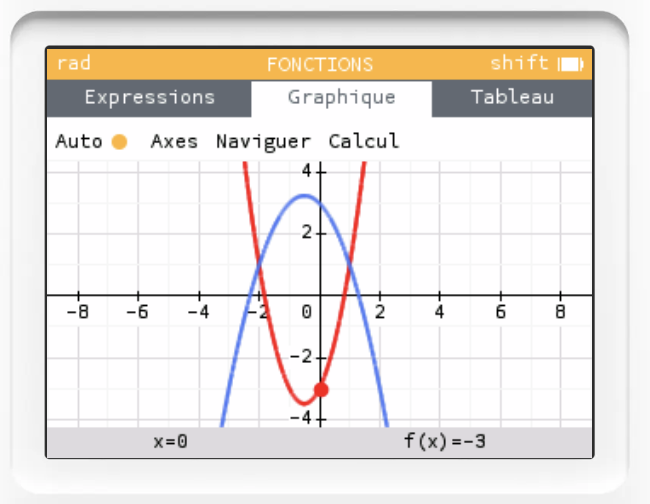
\includegraphics[scale=1]{1.03.06-Img01}
%	\end{center}
	\item Retrouver par le calcul les résultats précédents. \bareme{2}
\end{enumMet}



\end{document}

